\section{Training Data}
\label{sec:traning_data}
The method used for gesture recognition uses a comparison method that compare the input with a predefined set of training data, a more detailed view of the comparison method is described in \cref{sec:data_comparison}. This section will cover the training set in detail. Each defined ASL sign have three instances of JSON-files containing the training data for the ASL sign. \Cref{fig:training_data_diagram} shows a diagram of the progress of adding new instance of a gesture to the system.

\begin{figure}[!ht]
    \centering
    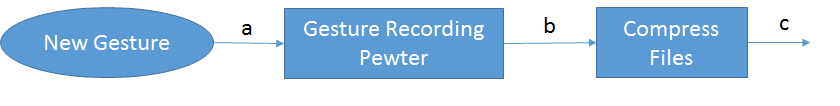
\includegraphics[height=1.6cm]{content/05-Methodology/images/step_creating_new_gesture.png}
    \caption[Training Data Diagram]{A stepwise diagram of the progress of recording new training instances. At step (a) we use Pewter to record the gesture, which returns data stored data in JSON-format at step (b). At step (c) the system provide a compression method for the raw JSON-files to ensure smaller file size.}
    \label{fig:training_data_diagram}
\end{figure}

\subsection{Data acquisition}
\label{subsec:data_acquisition}
Pewter is an open-source project developed by Ayushman Dash for acquisition, analysis and visualisation of raw data from the Myo Armband \cite{github:pewter}. Pewter is implemented using Node.js, which is a JavaScript runtime environment that is mostly used for developing web applications. The system provide a simple method to record raw data from the Myo armband, and store the recorded data in JSON-format. In addition it provide a visualisation page, where the data is represented in graphs.

\subsection{File Compression}
\label{subsec:file_compress}
Pewter described in \cref{subsec:data_acquisition} provide a simple method for recording gestures, but does not provide any methods to ensure a constant size of the recorded data. The recorded data have to be large enough to cover the gestures, but too large files causes the data analysis to be slow. 

All the raw files recorded from Pewter are recorded with an amount of unnecessary data, a margin to ensure that all the recorded data are within a certain time interval of approximately four seconds. The data for the actual gesture are below a time interval of two seconds. The implemented system provide a method to compress the JSON-files from Pewter to JSON-files with a constant data size given by a set time variable. The size of the data is not determined by the timestamps extractable from the raw JSON-files, but rather calculated using the sample-frequency of the sensors, using the same \cref{eq:data_size_eq} as for gesture recording.